\documentclass{article}

\usepackage[dblblindworkshop]{neurips_2026}
\workshoptitle{Who Verifies the Agents?}

\usepackage[utf8]{inputenc}
\usepackage[T1]{fontenc}
\usepackage{hyperref}
\usepackage{url}
\usepackage{booktabs}
\usepackage{amsfonts}
\usepackage{amsmath}
\usepackage{nicefrac}
\usepackage{microtype}
\usepackage{xcolor}
\usepackage{graphicx}
\usepackage{tabularx}
\usepackage{tikz}
\usetikzlibrary{arrows.meta,positioning,calc,fit}

\title{CounterFeint: Checking the Checker in a Three-Role Ad-Fraud Arena}

\author{%
  Abhijith Reddy Dasari \\
  Independent Researcher \\
  \texttt{abhijithreddydasari@gmail.com}
}

\begin{document}

\nolinenumbers
\raggedbottom
\maketitle

\begin{abstract}
Agent evaluations are as reliable as the verifiers that score them: weak verifiers can reward invalid behavior as success. We present CounterFeint, a replayable OpenEnv arena for testing verifier effectiveness in an ad-fraud environment. Three scripted roles share an ad marketplace: a \emph{Fraudster} proposes new ads, a budgeted \emph{Investigator} reviews them, and a deterministic \emph{Auditor} emits typed flags that affect both roles' rewards. Our paired protocol injects controlled defects into frozen trajectories, measures the resulting flags against sanitized controls, and then removes corresponding reward checks to measure their effect on the same trajectories. Locally checkable defects, including unsupported rationales and grader-trigger strings, are detected reliably. Notably, removing rationale checks increases Investigator reward by approximately $2.11$, while removing the plausibility gate increases Fraudster reward from $1.02$ to $4.50$ on gibberish ads. Other checks produce collateral flags or little reward change. CounterFeint provides a reproducible framework for testing whether verifier components detect specified defects and materially constrain reward in a scripted environment.
\end{abstract}

\section{Introduction}
\label{sec:intro}

Long-horizon agent evaluations often reduce an episode to a score produced by a grader, rubric, or LLM judge. An agent may obtain a high score by completing the task or exploiting a weakness in the measurement process \citep{skalse2022defining,pan2022effects}. Reliable evaluation therefore requires evidence that the verifier detects the relevant defects and constrains the reward.

Judge-reliability harnesses perturb benchmark traces to test LLM judges \citep{dev2026jrh,zhao2025onetoken}. Learned and agentic evaluators score other agents \citep{shi2026ajbench,luo2025agentauditor}, while symbolic checkers permit direct ablation of executable rules \citep{wang2026auditflow}. CounterFeint complements these approaches with a replayable OpenEnv arena \citep{openenv2026} where typed verifier outputs enter both sides' rewards. This structure supports a causal question on a frozen trace: does a check merely report a defect, or does it prevent that defect from increasing reward?

A scripted Fraudster and Investigator produce CPU-reproducible trajectories, while a deterministic Auditor reviews the output. Experimental ground truth comes from controlled trace mutations. Each mutation declares its expected flags before the Auditor executes separating the annotation process from the rules being evaluated.

We ask whether an injected defect produces a new flag relative to a sanitized control and whether removing the corresponding check increases reward on the same mutated trajectory. We call a check that changes reward a \emph{gate}; a flag without a material reward effect is a \emph{diagnostic}. Our contribution is the three-role environment and paired protocol for characterizing verifier behavior under scripted policies and a closed template distribution.

\section{Related Work}
\label{sec:related}

Prior work stress-tests LLM judges: Judge Reliability Harness builds validation suites by perturbing benchmark traces and scoring whether an LLM judge still agrees with the target label \citep{dev2026jrh}; One Token to Fool LLM-as-a-Judge shows that superficial ``master key'' strings can elicit a false-positive reward from generative graders \citep{zhao2025onetoken}. AJ-Bench and AgentAuditor evaluate agentic or memory-augmented judges of other agents \citep{shi2026ajbench,luo2025agentauditor}. Whereas AuditFlow separates LLM search from deterministic XBRL checks and reports that removing the checks collapses accuracy \citep{wang2026auditflow}. CounterFeint extends this ablation approach to a replayable OpenEnv interaction \citep{openenv2026}, using controlled defect injection to test flag detection and frozen-trajectory ablations to measure each check's effect on reward.

\section{Method}
\label{sec:method}

Each episode is a small marketplace managed by a shared OpenEnv referee. Catalog ads are sampled by seed from a closed template bank, and landing-page reports contain procedurally generated domain, age, SSL, and registrar fields. Three roles act on one queue: Fraudster and Investigator policies are scripted; the Auditor is a deterministic verifier. Figure~\ref{fig:protocol} summarizes the action space, written fields, and turn order for all three roles and see the Appendix~\ref{app:roles} for the full list of action fields.

\begin{figure}[t]
\centering
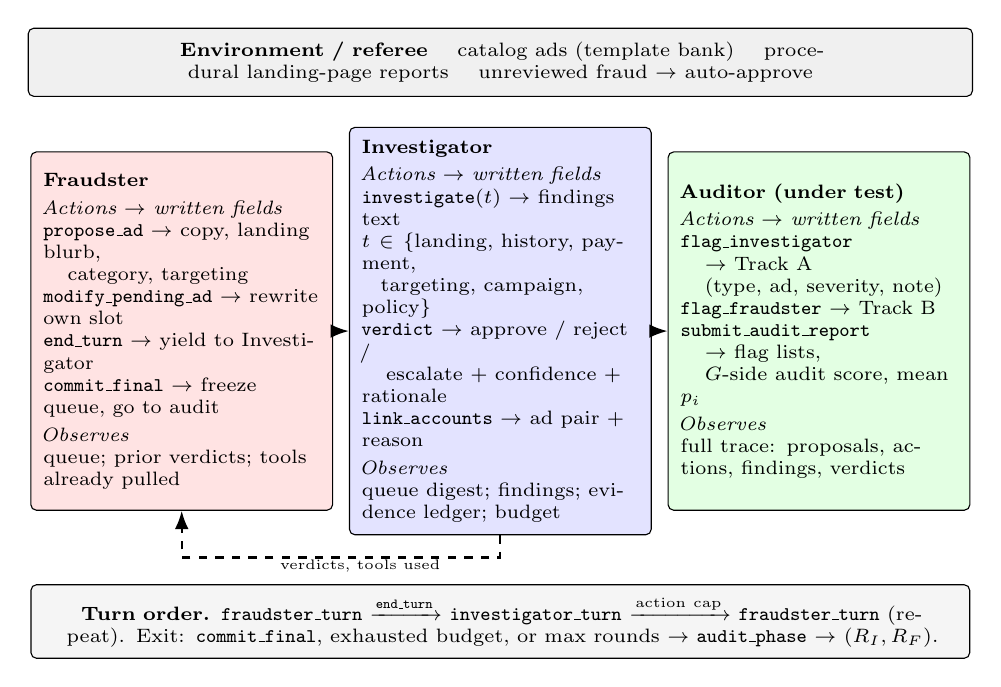
\begin{tikzpicture}[
  font=\scriptsize,
  arr/.style={-{Latex}, thick},
  darr/.style={-{Latex}, thick, dashed},
  envbox/.style={draw, rounded corners=2pt, fill=gray!12, inner sep=5pt, align=center, text width=0.96\linewidth},
  card/.style={draw, rounded corners=2pt, inner sep=4.5pt, align=left, text width=0.29\linewidth, font=\scriptsize, minimum height=4.55cm},
  strip/.style={draw, rounded corners=2pt, fill=black!4, inner sep=4pt, align=center, text width=0.96\linewidth, font=\scriptsize}
]
\node[envbox] (env) {%
  \textbf{Environment / referee} \quad catalog ads (template bank) \quad procedural landing-page reports \quad
  unreviewed fraud $\to$ auto-approve%
};
\node[card, fill=blue!11, below=0.38cm of env] (inv) {%
  \textbf{Investigator}\\[2pt]
  \textit{Actions $\to$ written fields}\\
  \texttt{investigate}($t$) $\to$ findings text\\
  $t\in\{$landing, history, payment,\\
  \hspace{0.85em}targeting, campaign, policy$\}$\\
  \texttt{verdict} $\to$ approve / reject /\\
  \hspace{1.1em}escalate + confidence + rationale\\
  \texttt{link\_accounts} $\to$ ad pair + reason\\[2pt]
  \textit{Observes}\\
  queue digest; findings; evidence ledger; budget
};
\node[card, fill=red!11, left=0.20cm of inv] (frd) {%
  \textbf{Fraudster}\\[2pt]
  \textit{Actions $\to$ written fields}\\
  \texttt{propose\_ad} $\to$ copy, landing blurb,\\
  \hspace{1.1em}category, targeting\\
  \texttt{modify\_pending\_ad} $\to$ rewrite own slot\\
  \texttt{end\_turn} $\to$ yield to Investigator\\
  \texttt{commit\_final} $\to$ freeze queue, go to audit\\[2pt]
  \textit{Observes}\\
  queue; prior verdicts; tools already pulled
};
\node[card, fill=green!11, right=0.20cm of inv] (aud) {%
  \textbf{Auditor (under test)}\\[2pt]
  \textit{Actions $\to$ written fields}\\
  \texttt{flag\_investigator}\\
  \hspace{1.1em}$\to$ Track~A\\
  \hspace{1.1em}(type, ad, severity, note)\\
  \texttt{flag\_fraudster} $\to$ Track~B\\
  \texttt{submit\_audit\_report}\\
  \hspace{1.1em}$\to$ flag lists,\\
  \hspace{1.1em}$G$-side audit score, mean $p_i$\\[2pt]
  \textit{Observes}\\
  full trace: proposals, actions, findings, verdicts
};
\draw[arr] (frd.east) -- (inv.west);
\draw[arr] (inv.east) -- (aud.west);
\draw[darr] (inv.south) -- ++(0,-0.28) -| node[pos=0.22, below, font=\tiny, inner sep=0.4pt] {verdicts, tools used} (frd.south);
\node[strip, below=0.62cm of inv] (ord) {%
  \textbf{Turn order.}
  \texttt{fraudster\_turn} $\xrightarrow{\texttt{end\_turn}}$ \texttt{investigator\_turn} $\xrightarrow{\text{action cap}}$ \texttt{fraudster\_turn} (repeat).
  Exit: \texttt{commit\_final}, exhausted budget, or max rounds $\to$ \texttt{audit\_phase} $\to$ $(R_I, R_F)$.
};
\end{tikzpicture}
\caption{\small Action spaces, written outputs, and turn-taking. The dashed edge shows the intra-episode feedback: the Fraudster observes Investigator verdicts and tool use before modifying remaining ads. Catalog ads and landing-page reports are environment-owned. All reported policies are scripted.}
\label{fig:protocol}
\end{figure}

\subsection{Episode protocol}
\label{sec:protocol}

The referee is a multi-phase state machine: \texttt{fraudster\_turn}, \texttt{investigator\_turn}, \texttt{audit\_phase}, \texttt{done}. On \texttt{fraudster\_turn} the agent may \texttt{propose\_ad}, \texttt{modify\_pending\_ad}, \texttt{end\_turn}, or \texttt{commit\_final}. Proposal count and per-turn actions are capped. The Fraudster observes the current queue, the Investigator's earlier verdicts, and the tools already used.

On \texttt{investigator\_turn}, the agent spends a limited budget on \texttt{investigate} (landing page, advertiser history, payment method, targeting overlap, campaign structure, or policy classifier), issues an approve, reject, or escalate \emph{verdict} with confidence in $[0,1]$ and a free-text rationale. It can also use \texttt{link\_accounts} to link two ads as a suspected ring. Unreviewed fraud is treated as approved. The episode returns to the Fraudster once the Investigator's per-turn action limit is reached, and proceeds to audit if the investigation budget is exhausted, every ad has a verdict, the Fraudster commits, or the round limit is hit.

After the live match the Auditor reads the full episode record and may \texttt{flag\_investigator}, \texttt{flag\_fraudster}, or \texttt{submit\_audit\_report}. Each flag records track, target ad, type, severity, and note. In this paper the Auditor is a deterministic script that emits typed Track A/B flags in one pass.

\subsection{Reward functions}
\label{sec:rewards}

Rewards are computed once at audit time from the frozen episode record and the Auditor flags. $R_I$ combines an outcome grade with a rationale bonus and a capped consistency penalty; $R_F$ credits each unrejected Fraudster ad, weighted by severity and Track~B plausibility.

$G\in[0,1]$ is the task grader over verdict correctness. For ad $i$, $p_i\in[0,1]$ is Track~B plausibility (gibberish, parameter mismatch, exact clones, grader-trigger strings) and $\mathrm{sev}_i$ is its severity; catalog ads with no Fraudster proposal have $p_i=1$. $\mathcal{V}_{\mathrm{clean}}$ is the set of verdicts with neither a \texttt{missing\_citation} nor an \texttt{incoherent\_rationale} flag, and $p_i$ in Equation~\ref{eq:inv} is the plausibility of the ad under that verdict. $\mathcal{U}$ is the set of Fraudster-proposed ads that were approved, escalated, or left unreviewed; $n_{\mathrm{incons}}$ counts \texttt{inconsistency} flags and $n_{\mathrm{banned}}$ counts rejected Fraudster ads.
\begin{align}
R_I
  &= G + 0.2 \sum_{v\in\mathcal{V}_{\mathrm{clean}}} p_i
   - 0.3\min\{n_{\mathrm{incons}},3\},
  \label{eq:inv}\\
R_F
  &= \sum_{i\in\mathcal{U}}\mathrm{sev}_i\, p_i
   - n_{\mathrm{banned}}.
  \label{eq:frd}
\end{align}

Track~A affects $R_I$ only. A verdict may still increase $G$ if the label is correct, but an unsupported or contradictory rationale excludes it from $\mathcal{V}_{\mathrm{clean}}$ and removes the $0.2$ bonus. The inconsistency penalty is applied to at most three flags. \texttt{Bias} and \texttt{miscalibration} are recorded and do not appear in Equation~\ref{eq:inv}.

Track~B affects $R_F$ directly and, through $p_i$, also scales the Investigator bonus. An unrejected gibberish ad remains in $\mathcal{U}$, yet $p_i \approx 0$ contributes no credit. Only a \texttt{reject} verdict removes a Fraudster ad from $\mathcal{U}$; catalog ads do not enter $R_F$. Table~\ref{tab:game} holds the trajectory fixed and either removes Track~A or sets $p_i=1$.

\subsection{Auditor}
\label{sec:auditor}

Track~A inspects Investigator verdicts for citation, coherence, calibration, consistency, and slice bias. Track~B inspects Fraudster ads for gibberish copy, parameter mismatches (copy, targeting, landing), exact template clones, and grader-trigger strings. Both are deterministic Python and take about $0.12$\,ms per episode on a laptop CPU.

\section{Experimental Protocol}
\label{sec:eval}

Unmodified scripted rollouts already raise frequent baseline flags (\texttt{missing\_citation} $0.99$, \texttt{parameter\_mismatch} $1.00$). Counting those as mutation-induced false positives would evaluate the baseline policy rather than the injected defect.

\textbf{Detection.} We first sanitize each trace so the target check is a true negative (aligned verdicts with cited evidence tokens; prosaic ad copy). Sanitization is procedural and does not query the Auditor. We then apply one controlled mutation whose expected $(\text{flag type},\text{ad id})$ keys we declare before audit, and we score only flags that are new relative to the sanitized control; any other new flag is a false positive. We exclude empty-expected trials from F1: three coverage gaps (investigation farming, unrelated account links, paraphrased template spam) and cases where the mutation cannot apply. Of $1{,}500$ trials, $1{,}148$ are applicable. We report $95\%$ intervals from $1{,}000$ bootstrap resamples (seed $0$).

\textbf{Reward ablation.} We ablate on the raw frozen trajectories. For each defect we mutate a trajectory once, hold ads, actions, findings, and verdicts fixed, and recompute reward under the full Auditor and a specified removal arm, without rerunning or retraining either policy.

\textbf{Scale.} Detection uses $100$ base episodes on marketplace sizes of $5$, $12$, and $20$ ads, with eight Investigator-side and seven Fraudster-side mutations. Ablations use a $30$-episode subset (seeds $11$--$20$ on each task). Appendix~\ref{app:details} lists mutation definitions, a worked example, intervals, and reproduction commands.

\section{Results}
\label{sec:results}

\paragraph{Detection.}
Table~\ref{tab:f1} reports paired-delta precision, recall, and F1. Locally checkable properties pass the implementation check: contradictory rationale and grader-trigger strings reach F1 $1.00$; missing citation $0.98$; parameter mismatch $0.86$. Gibberish has recall $1.00$ and precision $0.50$ (F1 $0.67$) because other surface mutations also look non-wordlike. Slice bias, miscalibration, inconsistency, and template repetition reach F1 $0.33$ to $0.44$, as they also fire on collateral mutations. The three uncovered mutations have hit rate $0$.

\begin{table}[ht]
\caption{\small Paired-delta detection, $100$ trajectories ($1{,}148$ applicable trials). New flags only vs.\ a sanitized control. Flag definitions and bootstrap $95\%$ F1 intervals: Appendix~\ref{app:details}.}
\label{tab:f1}
\centering
\small
\begin{tabular}{lccc}
\toprule
Flag & Prec. & Rec. & F1 \\
\midrule
\texttt{incoherent\_rationale} & $1.00$ & $1.00$ & $1.00$ \\
\texttt{branding\_anomaly} & $1.00$ & $1.00$ & $1.00$ \\
\texttt{missing\_citation} & $0.96$ & $1.00$ & $0.98$ \\
\texttt{parameter\_mismatch} & $0.75$ & $1.00$ & $0.86$ \\
\texttt{gibberish} & $0.50$ & $1.00$ & $0.67$ \\
\texttt{inconsistency} & $0.31$ & $0.74$ & $0.44$ \\
\texttt{miscalibration} & $0.26$ & $1.00$ & $0.41$ \\
\texttt{template\_repetition} & $0.20$ & $1.00$ & $0.33$ \\
\texttt{bias} & $0.20$ & $1.00$ & $0.33$ \\
\bottomrule
\end{tabular}
\end{table}

\paragraph{Reward influence.}
Table~\ref{tab:game} compares full and ablated reward on the same mutated trajectory. Investigator rows drop Track~A; Fraudster rows drop the plausibility gate. Appendix~\ref{app:details} defines each mutation and its declared flag. On missing-citation and contradictory-rationale mutations, Investigator reward rises from $1.01$ / $0.71$ to $3.13$ / $2.82$ ($\Delta \approx +2.11$); dropping only the matching check reproduces this lift. On gibberish ads, Fraudster reward rises from $1.02$ to $4.50$ ($\Delta \approx +3.48$). Grader-trigger tokens, country/TLD mismatch, category/targeting mismatch, and exact clones also pay more without the gate ($\Delta$ about $+1.9$ to $+2.5$). Overconfidence and slice bias barely move Investigator reward ($\Delta = +0.15$ and $+0.55$ for the whole track; $0$ for the matching check), and paraphrased spam barely moves Fraudster reward ($\Delta \approx +0.22$).

\begin{table}[ht]
\caption{\small Mean reward on the same raw mutated trajectory ($n=30$). Inv.\ rows drop Track~A; Frd.\ rows drop the plausibility gate. $\Delta$ is removed minus full. Mutation definitions and remaining rows: Appendix~\ref{app:details}.}
\label{tab:game}
\centering
\small
\begin{tabular}{llccc}
\toprule
Trace mutation & Role & Full & Removed & $\Delta$ \\
\midrule
missing citation & Inv. & $1.01$ & $3.13$ & $+2.11$ \\
contradictory rationale & Inv. & $0.71$ & $2.82$ & $+2.11$ \\
overconfidence & Inv. & $2.69$ & $2.84$ & $+0.15$ \\
slice bias & Inv. & $2.52$ & $3.07$ & $+0.55$ \\
gibberish ads & Frd. & $1.02$ & $4.50$ & $+3.48$ \\
grader-trigger tokens & Frd. & $1.97$ & $4.03$ & $+2.06$ \\
country / TLD mismatch & Frd. & $1.50$ & $4.03$ & $+2.53$ \\
template clones & Frd. & $1.74$ & $4.03$ & $+2.29$ \\
paraphrased spam & Frd. & $3.80$ & $4.03$ & $+0.22$ \\
\bottomrule
\end{tabular}
\end{table}

\section{Limitations and Conclusion}
\label{sec:limits}

The catalog is a closed template bank and both counterparties are scripted, so Table~\ref{tab:game} asks what the reward function pays once a check is removed, not whether a trained agent would find that hole. Investigation farming, unrelated links, and paraphrase remain invisible, and bias and calibration flags barely move reward. We release CounterFeint as a verifier-testing environment, not a production moderation stack.

It pairs detection with reward ablation on the same frozen trace, so we can tell gates from diagnostics. Exact checks detect their targeted defects and materially constrain reward, while noisier checks expose collateral flags and missing reward connections. These results demonstrate how an agent environment can test its measurement layer directly and report verifier weaknesses alongside successful gates.

\begin{ack}
Omitted in the anonymized submission.
\end{ack}

{\small
\begin{thebibliography}{10}

\bibitem[Skalse et al.(2022)]{skalse2022defining}
J.~Skalse, N.~Howe, D.~Krasheninnikov, and D.~Krueger.
\newblock Defining and characterizing reward gaming.
\newblock In \emph{Advances in Neural Information Processing Systems}, 2022.

\bibitem[Pan et al.(2022)]{pan2022effects}
A.~Pan, K.~Bhatia, and J.~Steinhardt.
\newblock The effects of reward misspecification: Mapping and mitigating misaligned models.
\newblock In \emph{International Conference on Learning Representations}, 2022.

\bibitem[Dev et al.(2026)]{dev2026jrh}
S.~Dev, A.~Sloan, J.~Kavner, N.~Kong, and M.~Sandler.
\newblock Judge reliability harness: Stress testing the reliability of {LLM} judges.
\newblock In \emph{{ICLR} Workshop on Agents in the Wild}, 2026.
\newblock arXiv:2603.05399.

\bibitem[Zhao et al.(2025)]{zhao2025onetoken}
Y.~Zhao, H.~Liu, D.~Yu, S.~Y.~Kung, M.~Chen, H.~Mi, and D.~Yu.
\newblock One token to fool {LLM}-as-a-judge.
\newblock In \emph{{NeurIPS} Workshop on Mathematical Reasoning and {AI}}, 2025.
\newblock arXiv:2507.08794.

\bibitem[Shi et al.(2026)]{shi2026ajbench}
W.~Shi, Y.~Wang, Y.~Zhao, Y.~Chen, F.~Feng, X.~Hao, X.~Su, Q.~Gu, H.~Su, X.~Cai, and X.~He.
\newblock {{AJ}-Bench}: Benchmarking agent-as-a-judge for environment-aware evaluation.
\newblock In \emph{Findings of the Association for Computational Linguistics}, 2026.
\newblock doi:10.18653/v1/2026.findings-acl.1269.

\bibitem[Luo et al.(2025)]{luo2025agentauditor}
H.~Luo, S.~Dai, C.~Ni, X.~Li, G.~Zhang, K.~Wang, T.~Liu, and H.~Salam.
\newblock {AgentAuditor}: Human-level safety and security evaluation for {LLM} agents.
\newblock In \emph{Advances in Neural Information Processing Systems}, 2025.
\newblock arXiv:2506.00641.

\bibitem[Wang et al.(2026)]{wang2026auditflow}
Y.~Wang, X.~Ai, J.~Patel, X.~Peng, F.~Mo, Y.~Cao, H.~Li, M.~Cao, L.~Qian, and V.~Guti\'{e}rrez-Basulto.
\newblock {AuditFlow}: Executable symbolic environments for structured financial reporting verification.
\newblock arXiv:2606.03031, 2026.

\bibitem[Hugging Face(2026)]{openenv2026}
Hugging Face.
\newblock {OpenEnv}: Agentic execution environments.
\newblock \url{https://github.com/huggingface/openenv}, 2026.

\end{thebibliography}
}

\appendix

\section*{Appendix}
This appendix records the role action spaces summarized in Figure~\ref{fig:protocol}, defines each controlled trace mutation, reports bootstrap intervals and additional reward ablations, and gives the command used to reproduce Tables~\ref{tab:f1} and~\ref{tab:game}.

\section{Roles and action spaces}
\label{app:roles}

On \texttt{fraudster\_turn} the agent may \texttt{propose\_ad} (copy, landing-page blurb, category, targeting), \texttt{modify\_pending\_ad} on its own slots, \texttt{end\_turn}, or \texttt{commit\_final} (no further proposals; jump to audit). It observes the queue, every Investigator verdict so far, and which tools have already been pulled.

On \texttt{investigator\_turn} the agent spends a limited budget on \texttt{investigate} with a target in $\{\texttt{landing\_page}$, $\texttt{advertiser\_history}$, $\texttt{payment\_method}$, $\texttt{targeting\_overlap}$, $\texttt{campaign\_structure}$, $\texttt{policy\_classifier}\}$; issues a \texttt{verdict} in $\{\texttt{approve}$, $\texttt{reject}$, $\texttt{escalate}\}$ with confidence in $[0,1]$ and a free-text rationale; or \texttt{link\_accounts} two ads. Findings text is written into the evidence ledger. Unreviewed fraud is auto-approved.

In \texttt{audit\_phase} the Auditor may \texttt{flag\_investigator} (Track~A: type, ad, severity, note), \texttt{flag\_fraudster} (Track~B), or \texttt{submit\_audit\_report} (flag lists, $G$-side audit score, mean $p_i$). It observes the full trace: proposals, actions, findings, and verdicts. Catalog ads and landing-page reports are environment-owned.

\section{Experimental details}
\label{app:details}

\paragraph{Worked example.}
Sanitize a page that reports a valid certificate and an \texttt{approve} verdict whose rationale cites an evidence token. The mutation appends ``no SSL / phishing, nevertheless approve.'' Expected new flag: \texttt{incoherent\_rationale} on that ad. Detection F1 is $1.00$. Hold the mutated trace fixed and drop Track~A: mean $R_I$ moves from $0.71$ to $2.82$.

\subsection{Controlled trace mutations}

Each constructor rewrites a frozen trace and declares the flag that should appear as a new signal. Table~\ref{tab:mutations} summarizes the rewrite; the notes below state what the name means.

\paragraph{Investigator-side mutations.}
\texttt{Missing citation} replaces the verdict rationale with text that cites no token from the findings. \texttt{Fabricated citation} inserts rationale tokens that do not appear in the findings; both declare \texttt{missing\_citation}. \texttt{Contradictory rationale} appends red-flag language (for example, ``no SSL / phishing'') to an approval, declaring \texttt{incoherent\_rationale}. \texttt{Overconfidence} assigns high confidence to deliberately incorrect verdicts and declares \texttt{miscalibration}. \texttt{Inconsistent verdicts} gives opposing labels to comparable ads and declares \texttt{inconsistency}. \texttt{Slice bias} forces systematic errors on one product category (here, category buckets rather than country) and declares \texttt{bias}. \texttt{Investigation farming} prepends repeated \texttt{investigate} actions, and \texttt{unrelated links} adds unsupported \texttt{link\_accounts} records; both declare an empty expected set because the current Auditor has no matching flag.

\paragraph{Fraudster-side mutations.}
\texttt{Gibberish ads} replace copy with random non-wordlike text and declare \texttt{gibberish}. \texttt{Grader-trigger tokens} insert scorer-facing identifiers and declare \texttt{branding\_anomaly}. \texttt{Country/TLD mismatch} pairs US-oriented copy with a conflicting top-level domain. \texttt{Category/targeting mismatch} pairs a high-risk category with incompatible targeting. \texttt{Internal inconsistency} pairs a high-risk category with incompatible product copy. Those three declare \texttt{parameter\_mismatch} (country/TLD also declares \texttt{branding\_anomaly}). \texttt{Template spam} duplicates exact ad copy and declares \texttt{template\_repetition}. \texttt{Paraphrased spam} inserts near-duplicate paraphrases and declares an empty expected set (novelty miss).

\begin{table}[ht]
\caption{\small Mutations applied after trajectory generation. An empty expected set denotes a documented coverage gap.}
\label{tab:mutations}
\centering
\scriptsize
\begin{tabularx}{\linewidth}{l l X l}
\toprule
Side & Mutation & Trace modification & Declared flag \\
\midrule
Inv. & missing citation & Replace rationale with text that cites no finding token & \texttt{missing\_citation} \\
Inv. & fabricated citation & Insert fabricated rationale tokens disjoint from findings & \texttt{missing\_citation} \\
Inv. & contradictory rationale & Append red-flag evidence to an approval rationale & \texttt{incoherent\_rationale} \\
Inv. & overconfidence & Assign high confidence to deliberately incorrect verdicts & \texttt{miscalibration} \\
Inv. & inconsistent verdicts & Give opposing verdicts to comparable ads & \texttt{inconsistency} \\
Inv. & slice bias & Force systematic errors on one category slice & \texttt{bias} \\
Inv. & investigation farming & Prepend repeated investigation actions & empty \\
Inv. & unrelated links & Add unsupported advertiser-account links & empty \\
\midrule
Frd. & gibberish ads & Replace copy with random non-wordlike text & \texttt{gibberish} \\
Frd. & grader-trigger tokens & Insert identifiers copied from scorer-facing fields & \texttt{branding\_anomaly} \\
Frd. & country/TLD mismatch & Pair US-oriented copy with a conflicting top-level domain & \texttt{parameter\_mismatch}, \texttt{branding\_anomaly} \\
Frd. & category/target mismatch & Pair a high-risk category with incompatible targeting & \texttt{parameter\_mismatch} \\
Frd. & template spam & Duplicate exact ad copy across proposals & \texttt{template\_repetition} \\
Frd. & paraphrased spam & Insert near-duplicate paraphrases of a template & empty \\
Frd. & internal inconsistency & Pair a high-risk category with incompatible product copy & \texttt{parameter\_mismatch} \\
\bottomrule
\end{tabularx}
\end{table}

\subsection{Detection details}

\paragraph{Mutation hit rates.}
Rates over the $100$ base trajectories are $1.00$ for missing citation, fabricated citation, contradictory rationale, gibberish, grader-trigger tokens, country/TLD mismatch, category/targeting mismatch, and internal inconsistency. Rates are $0.88$ for overconfidence, $0.74$ for inconsistent verdicts, $0.60$ for slice bias, and $0.67$ for template spam. Investigation farming, unrelated links, and paraphrased spam have hit rate $0$ because the current Auditor has no corresponding flag. These three constructors declare an empty expected set and are reported as coverage gaps rather than included in F1.

\paragraph{Bootstrap intervals.}
{\raggedright
Trajectory-level $95\%$ F1 intervals from $1{,}000$ bootstrap samples are $[1.00,1.00]$ for \texttt{branding\_anomaly} and \texttt{incoherent\_rationale}, $[0.98,0.98]$ for \texttt{missing\_citation}, $[0.86,0.86]$ for \texttt{parameter\_mismatch}, $[0.66,0.67]$ for \texttt{gibberish}, $[0.43,0.44]$ for \texttt{inconsistency}, $[0.41,0.41]$ for \texttt{miscalibration}, $[0.33,0.34]$ for \texttt{template\_repetition}, and $[0.33,0.33]$ for \texttt{bias}.\par}

\paragraph{Clean-control rates.}
{\raggedright
On unmodified scripted trajectories, rates are \texttt{missing\_citation} $0.99$, \texttt{parameter\_mismatch} $1.00$, \texttt{miscalibration} $0.58$, \texttt{bias} $0.45$, \texttt{gibberish} $0.44$, \texttt{inconsistency} $0.39$, and \texttt{template\_repetition} $0.05$.\par}

\subsection{Additional reward ablations}

The main table presents representative rows. Additional Fraudster-side full-to-no-gate changes are $2.14$ to $4.03$ for category/targeting mismatch ($\Delta=+1.88$) and $1.77$ to $4.03$ for internal inconsistency ($\Delta=+2.26$). Fabricated citation changes Investigator reward from $1.01$ to $3.13$ when Track~A is removed ($\Delta=+2.11$). Removing only the matching check yields $\Delta=+0.49$ for inconsistent verdicts, $+0.65$ for gibberish, $+1.65$ for grader-trigger tokens, $+0.06$ for country/TLD mismatch, $+1.83$ for category/targeting mismatch, and $+2.01$ for exact template spam. Matching-check removal yields $0$ for overconfidence and slice bias.

\subsection{Reproduction and compute}

The complete deterministic experiment suite can be reproduced from the repository root with:
\begin{quote}
\small\texttt{python -m counterfeint.experiments paper1}
\end{quote}
Detection uses task-specific seed ranges $11$--$50$, $11$--$45$, and $11$--$35$, giving $100$ trajectories. Ablations use seeds $11$--$20$ for each of the three tasks. The deterministic audit requires approximately $0.12$\,ms per episode on a laptop CPU. Tables~\ref{tab:f1} and~\ref{tab:game} require no GPU and involve no model training.

\newpage
\section*{NeurIPS Paper Checklist}

\begin{enumerate}

\item {\bf Claims}
    \item[] Question: Do the main claims made in the abstract and introduction accurately reflect the paper's contributions and scope?
    \item[] Answer: \answerYes{}
    \item[] Justification: The abstract and Section~\ref{sec:intro} state the two questions, distinguish detection from reward influence, and scope the evidence to scripted policies and a closed template distribution. The numerical claims match Tables~\ref{tab:f1} and~\ref{tab:game}.
    \item[] Guidelines:
    \begin{itemize}
        \item The answer \answerNA{} means that the abstract and introduction do not include the claims made in the paper.
        \item The abstract and/or introduction should clearly state the claims made, including the contributions made in the paper and important assumptions and limitations. A \answerNo{} or \answerNA{} answer to this question will not be perceived well by the reviewers.
        \item The claims made should match theoretical and experimental results, and reflect how much the results can be expected to generalize to other settings.
        \item It is fine to include aspirational goals as motivation as long as it is clear that these goals are not attained by the paper.
    \end{itemize}

\item {\bf Limitations}
    \item[] Question: Does the paper discuss the limitations of the work performed by the authors?
    \item[] Answer: \answerYes{}
    \item[] Justification: Section~\ref{sec:limits} covers template ads, scripted counterparties, noisy checks, coverage gaps, and the counterfactual nature of the ablation results.
    \item[] Guidelines:
    \begin{itemize}
        \item The answer \answerNA{} means that the paper has no limitation while the answer \answerNo{} means that the paper has limitations, but those are not discussed in the paper.
        \item The authors are encouraged to create a separate ``Limitations'' section in their paper.
        \item The paper should point out any strong assumptions and how robust the results are to violations of these assumptions (e.g., independence assumptions, noiseless settings, model well-specification, asymptotic approximations only holding locally). The authors should reflect on how these assumptions might be violated in practice and what the implications would be.
        \item The authors should reflect on the scope of the claims made, e.g., if the approach was only tested on a few datasets or with a few runs. In general, empirical results often depend on implicit assumptions, which should be articulated.
        \item The authors should reflect on the factors that influence the performance of the approach. For example, a facial recognition algorithm may perform poorly when image resolution is low or images are taken in low lighting. Or a speech-to-text system might not be used reliably to provide closed captions for online lectures because it fails to handle technical jargon.
        \item The authors should discuss the computational efficiency of the proposed algorithms and how they scale with dataset size.
        \item If applicable, the authors should discuss possible limitations of their approach to address problems of privacy and fairness.
        \item While the authors might fear that complete honesty about limitations might be used by reviewers as grounds for rejection, a worse outcome might be that reviewers discover limitations that aren't acknowledged in the paper. The authors should use their best judgment and recognize that individual actions in favor of transparency play an important role in developing norms that preserve the integrity of the community. Reviewers will be specifically instructed to not penalize honesty concerning limitations.
    \end{itemize}

\item {\bf Theory assumptions and proofs}
    \item[] Question: For each theoretical result, does the paper provide the full set of assumptions and a complete (and correct) proof?
    \item[] Answer: \answerNA{}
    \item[] Justification: The paper is empirical. There are no theorems.
    \item[] Guidelines:
    \begin{itemize}
        \item The answer \answerNA{} means that the paper does not include theoretical results.
        \item All the theorems, formulas, and proofs in the paper should be numbered and cross-referenced.
        \item All assumptions should be clearly stated or referenced in the statement of any theorems.
        \item The proofs can either appear in the main paper or the supplemental material, but if they appear in the supplemental material, the authors are encouraged to provide a short proof sketch to provide intuition.
        \item Inversely, any informal proof provided in the core of the paper should be complemented by formal proofs provided in appendix or supplemental material.
        \item Theorems and Lemmas that the proof relies upon should be properly referenced.
    \end{itemize}

\item {\bf Experimental result reproducibility}
    \item[] Question: Does the paper fully disclose all the information needed to reproduce the main experimental results of the paper to the extent that it affects the main claims and/or conclusions of the paper (regardless of whether the code and data are provided or not)?
    \item[] Answer: \answerYes{}
    \item[] Justification: Sections~\ref{sec:method} and~\ref{sec:eval} distinguish the sanitized detection protocol from raw-trajectory reward ablation and specify roles, rewards, seeds, mutations, and the (flag type, ad id) scoring rule. The appendix gives the reproduction command and seed ranges. An anonymized code zip is included as supplementary material.
    \item[] Guidelines:
    \begin{itemize}
        \item The answer \answerNA{} means that the paper does not include experiments.
        \item If the paper includes experiments, a \answerNo{} answer to this question will not be perceived well by the reviewers: Making the paper reproducible is important, regardless of whether the code and data are provided or not.
        \item If the contribution is a dataset and\slash or model, the authors should describe the steps taken to make their results reproducible or verifiable.
        \item Depending on the contribution, reproducibility can be accomplished in various ways. For example, if the contribution is a novel architecture, describing the architecture fully might suffice, or if the contribution is a specific model and empirical evaluation, it may be necessary to either make it possible for others to replicate the model with the same dataset, or provide access to the model. In general. releasing code and data is often one good way to accomplish this, but reproducibility can also be provided via detailed instructions for how to replicate the results, access to a hosted model (e.g., in the case of a large language model), releasing of a model checkpoint, or other means that are appropriate to the research performed.
        \item While NeurIPS does not require releasing code, the conference does require all submissions to provide some reasonable avenue for reproducibility, which may depend on the nature of the contribution.
    \end{itemize}

\item {\bf Open access to data and code}
    \item[] Question: Does the paper provide open access to the data and code, with sufficient instructions to faithfully reproduce the main experimental results, as described in supplemental material?
    \item[] Answer: \answerYes{}
    \item[] Justification: An anonymized supplementary zip includes the environment, Auditor, mutation suite, table-generation scripts, and the saved Table~1/2 reports. Trajectories are rebuilt from seeds via \texttt{python -m counterfeint.experiments paper1}.
    \item[] Guidelines:
    \begin{itemize}
        \item The answer \answerNA{} means that paper does not include experiments requiring code.
        \item Please see the NeurIPS code and data submission guidelines (\url{https://neurips.cc/public/guides/CodeSubmissionPolicy}) for more details.
        \item While we encourage the release of code and data, we understand that this might not be possible, so \answerNo{} is an acceptable answer. Papers cannot be rejected simply for not including code, unless this is central to the contribution (e.g., for a new open-source benchmark).
        \item The instructions should contain the exact command and environment needed to run to reproduce the results.
        \item At submission time, to preserve anonymity, the authors should release anonymized versions (if applicable).
    \end{itemize}

\item {\bf Experimental setting/details}
    \item[] Question: Does the paper specify all the training and test details (e.g., data splits, hyperparameters, how they were chosen, type of optimizer) necessary to understand the results?
    \item[] Answer: \answerYes{}
    \item[] Justification: There is no training. Section~\ref{sec:eval} and the appendix list episode counts, seeds, attacks, and the paired protocol.
    \item[] Guidelines:
    \begin{itemize}
        \item The answer \answerNA{} means that the paper does not include experiments.
        \item The experimental setting should be presented in the core of the paper to a level of detail that is necessary to appreciate the results and make sense of them.
        \item The full details can be provided either with the code, in appendix, or as supplemental material.
    \end{itemize}

\item {\bf Experiment statistical significance}
    \item[] Question: Does the paper report error bars suitably and correctly defined or other appropriate information about the statistical significance of the experiments?
    \item[] Answer: \answerYes{}
    \item[] Justification: Detection F1 uses trajectory-level bootstrap $95\%$ intervals (Section~\ref{sec:eval}, Table~\ref{tab:f1} caption). Ablation rewards are means over a fixed $30$-episode subset.
    \item[] Guidelines:
    \begin{itemize}
        \item The answer \answerNA{} means that the paper does not include experiments.
        \item The authors should answer \answerYes{} if the results are accompanied by error bars, confidence intervals, or statistical significance tests, at least for the experiments that support the main claims of the paper.
        \item The factors of variability that the error bars are capturing should be clearly stated (for example, train/test split, initialization, random drawing of some parameter, or overall run with given experimental conditions).
        \item The method for calculating the error bars should be explained (closed form formula, call to a library function, bootstrap, etc.).
    \end{itemize}

\item {\bf Experiments compute resources}
    \item[] Question: For each experiment, does the paper provide sufficient information on the computer resources (type of compute workers, memory, time of execution) needed to reproduce the experiments?
    \item[] Answer: \answerYes{}
    \item[] Justification: Main tables are CPU-only. Appendix reports $\approx 0.12$\,ms per deterministic audit. No GPU is required for the reported claims.
    \item[] Guidelines:
    \begin{itemize}
        \item The answer \answerNA{} means that the paper does not include experiments.
        \item The paper should indicate the type of compute workers CPU or GPU, internal cluster, or cloud provider, including relevant memory and storage.
        \item The paper should provide the amount of compute required for each of the individual experimental runs as well as estimate the total compute.
        \item The paper should disclose whether the full research project required more compute than the experiments reported in the paper (e.g., preliminary or failed experiments that didn't make it into the paper).
    \end{itemize}

\item {\bf Code of ethics}
    \item[] Question: Does the research conducted in the paper conform, in every respect, with the NeurIPS Code of Ethics \url{https://neurips.cc/public/EthicsGuidelines}?
    \item[] Answer: \answerYes{}
    \item[] Justification: Work is a synthetic simulator with no human subjects. Section~\ref{sec:limits} scopes the release as a verifier-testing environment, not a production moderation stack.
    \item[] Guidelines:
    \begin{itemize}
        \item The answer \answerNA{} means that the authors have not reviewed the NeurIPS Code of Ethics.
        \item If the authors answer \answerNo{}, they should explain the special circumstances that require a deviation from the Code of Ethics.
        \item The authors should make sure to preserve anonymity (e.g., if there is a special consideration due to laws or regulations in their jurisdiction).
    \end{itemize}

\item {\bf Broader impacts}
    \item[] Question: Does the paper discuss both potential positive societal impacts and negative societal impacts of the work performed?
    \item[] Answer: \answerYes{}
    \item[] Justification: Positive: a replayable place to test verifier components before they are treated as measurement. Negative: the risk of reading a template simulator as production evidence (Section~\ref{sec:limits}).
    \item[] Guidelines:
    \begin{itemize}
        \item The answer \answerNA{} means that there is no societal impact of the work performed.
        \item If the authors answer \answerNA{} or \answerNo{}, they should explain why their work has no societal impact or why the paper does not address societal impact.
        \item Examples of negative societal impacts include potential malicious or unintended uses (e.g., disinformation, generating fake profiles, surveillance), fairness considerations, privacy considerations, and security considerations.
    \end{itemize}

\item {\bf Safeguards}
    \item[] Question: Does the paper describe safeguards that have been put in place for responsible release of data or models that have a high risk for misuse (e.g., pre-trained language models, image generators, or scraped datasets)?
    \item[] Answer: \answerNA{}
    \item[] Justification: No pretrained generator or scraped user data is released. Ads are short synthetic templates.
    \item[] Guidelines:
    \begin{itemize}
        \item The answer \answerNA{} means that the paper poses no such risks.
        \item Released models that have a high risk for misuse or dual-use should be released with necessary safeguards to allow for controlled use of the model.
        \item Datasets that have been scraped from the Internet could pose safety risks. The authors should describe how they avoided releasing unsafe images.
    \end{itemize}

\item {\bf Licenses for existing assets}
    \item[] Question: Are the creators or original owners of assets (e.g., code, data, models), used in the paper, properly credited and are the license and terms of use explicitly mentioned and properly respected?
    \item[] Answer: \answerYes{}
    \item[] Justification: OpenEnv is cited \citep{openenv2026}. No third-party scraped ad corpus is used.
    \item[] Guidelines:
    \begin{itemize}
        \item The answer \answerNA{} means that the paper does not use existing assets.
        \item The authors should cite the original paper that produced the code package or dataset.
        \item The name of the license (e.g., CC-BY 4.0) should be included for each asset.
    \end{itemize}

\item {\bf New assets}
    \item[] Question: Are new assets introduced in the paper well documented and is the documentation provided alongside the assets?
    \item[] Answer: \answerYes{}
    \item[] Justification: The environment, Auditor, mutation suite, and experiment protocol are specified in Sections~\ref{sec:method} and~\ref{sec:eval} and Appendix~\ref{app:details}. An anonymized copy ships in the supplementary zip.
    \item[] Guidelines:
    \begin{itemize}
        \item The answer \answerNA{} means that the paper does not release new assets.
        \item Researchers should communicate the details of the dataset\slash code\slash model as part of their submissions via structured templates.
        \item At submission time, remember to anonymize your assets (if applicable).
    \end{itemize}

\item {\bf Crowdsourcing and research with human subjects}
    \item[] Question: For crowdsourcing experiments and research with human subjects, does the paper include the full text of instructions given to participants and screenshots, if applicable, as well as details about compensation (if any)?
    \item[] Answer: \answerNA{}
    \item[] Justification: No crowdsourcing and no human-subject study.
    \item[] Guidelines:
    \begin{itemize}
        \item The answer \answerNA{} means that the paper does not involve crowdsourcing nor research with human subjects.
        \item Including this information in the supplemental material is fine, but if the main contribution of the paper involves human subjects, then as much detail as possible should be included in the main paper.
    \end{itemize}

\item {\bf Institutional review board (IRB) approvals or equivalent for research with human subjects}
    \item[] Question: Does the paper describe potential risks incurred by study participants, whether such risks were disclosed to the subjects, and whether Institutional Review Board (IRB) approvals (or an equivalent approval/review based on the requirements of your country or institution) were obtained?
    \item[] Answer: \answerNA{}
    \item[] Justification: No human-subject research.
    \item[] Guidelines:
    \begin{itemize}
        \item The answer \answerNA{} means that the paper does not involve crowdsourcing nor research with human subjects.
        \item Depending on the country in which research is conducted, IRB approval (or equivalent) may be required for any human subjects research.
    \end{itemize}

\item {\bf Declaration of LLM usage}
    \item[] Question: Does the paper describe the usage of LLMs if it is an important, original, or non-standard component of the core methods in this research? Note that if the LLM is used only for writing, editing, or formatting purposes and does \emph{not} impact the core methodology, scientific rigor, or originality of the research, declaration is not required.
    \item[] Answer: \answerNA{}
    \item[] Justification: The Auditor and both counterparties in the reported experiments are deterministic scripts. No LLM is part of the core method.
    \item[] Guidelines:
    \begin{itemize}
        \item The answer \answerNA{} means that the core method development in this research does not involve LLMs as any important, original, or non-standard components.
        \item Please refer to our LLM policy in the NeurIPS handbook for what should or should not be described.
    \end{itemize}

\end{enumerate}


\end{document}
